\documentclass[aspectratio=169,11pt]{beamer}

% Kort, folkelig deck for Arendalsgata 2026 (25 min, Sagene samfunnshus).
% Tema: Metropolis, uten seksjonssider.
\usetheme{metropolis}
\metroset{numbering=none, progressbar=foot, sectionpage=none}

\usepackage[utf8]{inputenc}
\usepackage[T1]{fontenc}
\usepackage[norsk]{babel}
\usepackage{booktabs}
\usepackage{array}
\usepackage{tikz}
\usepackage{xcolor}
\usepackage{colortbl}
\usepackage{amsmath}
\usepackage{ragged2e}

% Delte stiler fra de andre deckene
% Shared TikZ styles and macros for the exposure-mapping slides.

\usetikzlibrary{positioning, arrows.meta, shapes.geometric, fit, backgrounds, calc}

% Color palette: one color per code system.
\definecolor{cSTYRK}{HTML}{1F4E79}   % STYRK / overlapping ISCO codes: deep blue
\definecolor{cSOC10}{HTML}{C55A11}   % SOC 2010: orange
\definecolor{cSOC18}{HTML}{ED7D31}   % SOC 2018: light orange
\definecolor{cTASK}{HTML}{548235}    % O*NET task: green
\definecolor{cABIL}{HTML}{7030A0}    % O*NET ability: purple
\definecolor{cSCORE}{HTML}{000000}   % final score: black

% A code-system box: \codebox{color}{label}{code}{title}
%   label = "STYRK-08", "SOC 2010", "ISCO-08", ...
%   code  = "2262", "29-1051", ...
%   title = "Pharmacists" / Norwegian name
\tikzset{
  codebox/.style={
    draw=#1, line width=0.6pt,
    rounded corners=2pt,
    inner sep=3pt,
    fill=#1!8,
    text=black,
    align=center,
    minimum width=2.4cm,
    minimum height=0.85cm,
    font=\footnotesize
  },
  taskbox/.style={
    codebox=cTASK,
    minimum width=4cm,
    align=left,
    font=\scriptsize
  },
  chain/.style={
    -{Stealth[length=2mm,width=1.6mm]},
    line width=0.8pt,
    draw=black!50
  },
  arrowlabel/.style={
    font=\scriptsize\itshape,
    text=black!60,
    midway,
    above=2pt,
    fill=white,
    inner sep=1pt
  }
}

% \cbox{color}{label}{code}{title}
\newcommand{\cbox}[4]{%
  \begin{tabular}{c}%
    {\scriptsize\color{#1!85!black}\textbf{#2}}\\[-1pt]%
    {\bfseries #3}\\[-1pt]%
    {\scriptsize #4}%
  \end{tabular}%
}

% Task-table row highlights for Eloundou task scores (requires colortbl).
%   \rR{task}{E}{beta} = score 1.0 row (E_1), light red
%   \rO{task}{E}{beta} = score 0.5 row (E_2), light orange
% Score 0.0 rows are written plain (no cellcolor).
\definecolor{taskRed}{HTML}{FBDADA}
\definecolor{taskOrange}{HTML}{FFE8CC}
\newcommand{\rR}[3]{\cellcolor{taskRed}#1 & \cellcolor{taskRed}#2 & \cellcolor{taskRed}#3}
\newcommand{\rO}[3]{\cellcolor{taskOrange}#1 & \cellcolor{taskOrange}#2 & \cellcolor{taskOrange}#3}

% Palett og TikZ-stiler for illustrasjonsslidene.
% Fargene er hentet fra den private pptx-decken (sam-semesteråpning).
% Hver tekstblokk er en egen node med font=-opsjon, slik at linjeavstanden
% følger fontstørrelsen (fontbytte inne i en node gir feil baselineskip).

\definecolor{illBg}{HTML}{F7F9FC}
\definecolor{illInk}{HTML}{10243E}
\definecolor{illGray}{HTML}{516274}
\definecolor{illPanel}{HTML}{E7EDF4}
\definecolor{illBlue}{HTML}{2F6FB0}
\definecolor{illTeal}{HTML}{2A9D8F}
\definecolor{illOrange}{HTML}{F4A261}
\definecolor{illRed}{HTML}{D65A5A}
\definecolor{illPurple}{HTML}{7566C8}

\newcounter{illnode}

% Kort med farget aksentstripe til venstre:
%   \illcard{(x,y)}{farge}{OVERLINJE}{Tittel}{brødtekst}
% Tegnes inne i en tikzpicture. Kortet er ca. 4.3 cm bredt.
\newcommand{\illcard}[5]{%
  \stepcounter{illnode}%
  \fill[#2] #1 rectangle ($#1+(0.09,-3.6)$);
  \node[anchor=north west, text width=3.9cm, inner sep=0pt,
        font=\scriptsize\bfseries, text=#2]
        (illn\theillnode a) at ($#1+(0.35,-0.05)$) {#3};
  \node[anchor=north west, text width=3.9cm, inner sep=0pt,
        font=\bfseries, text=illInk]
        (illn\theillnode b) at ($(illn\theillnode a.south west)+(0,-0.2)$) {#4};
  \node[anchor=north west, text width=3.9cm, inner sep=0pt,
        font=\scriptsize, text=illGray]
        at ($(illn\theillnode b.south west)+(0,-0.25)$) {#5};
}

% Mørk banner med hvit tekst over hele tekstbredden:
%   \illbanner{tekst}
\newcommand{\illbanner}[1]{%
  \begin{tikzpicture}
    \node[fill=illInk, rounded corners=5pt, text=white, font=\bfseries,
          minimum width=\textwidth, minimum height=0.95cm,
          text width=0.92\textwidth, align=center, inner ysep=6pt] {#1};
  \end{tikzpicture}}

% Trinnkort i prosesskjeden:
%   \illstep{(x,y)}{nr}{Tittel}{spørsmål}         (uten fyll)
%   \illstepx{(x,y)}{nr}{Tittel}{spørsmål}        (uthevet, lys blå plate)
\newcommand{\illstep}[4]{%
  \stepcounter{illnode}%
  \node[anchor=north west, text width=2.6cm, inner sep=0pt,
        font=\small\bfseries, text=illBlue]
        (illn\theillnode a) at ($#1+(0.12,-0.15)$) {#2};
  \node[anchor=north west, text width=2.6cm, inner sep=0pt,
        font=\bfseries, text=illInk]
        (illn\theillnode b) at ($(illn\theillnode a.south west)+(0,-0.18)$) {#3};
  \node[anchor=north west, text width=2.6cm, inner sep=0pt,
        font=\footnotesize, text=illGray]
        at ($(illn\theillnode b.south west)+(0,-0.22)$) {#4};
}
\newcommand{\illstepx}[4]{%
  \fill[illPanel, rounded corners=6pt] ($#1+(-0.18,0.35)$) rectangle ($#1+(2.95,-3.3)$);
  \illstep{#1}{#2}{#3}{#4}%
}
% Pil mellom trinnkort: \illarrow{(x,y)}
\newcommand{\illarrow}[1]{%
  \fill[illGray!70] ($#1+(0,0.09)$) -- ($#1+(0.34,-0.07)$) -- ($#1+(0,-0.23)$) -- cycle;
}

% E-rad for eksponeringskategoriene:
%   \illerow{(x,y)}{farge}{E0}{Skår: 0}{Tittel}{beskrivelse}
\newcommand{\illerow}[6]{%
  \fill[#2] #1 rectangle ($#1+(0.09,-1.55)$);
  \node[anchor=north west, inner sep=0pt, font=\large\bfseries, text=#2]
        at ($#1+(0.35,-0.02)$) {#3};
  \node[anchor=north west, inner sep=0pt, font=\footnotesize\bfseries, text=illGray]
        at ($#1+(1.35,-0.09)$) {#4};
  \node[anchor=north west, inner sep=0pt, font=\bfseries, text=illInk]
        at ($#1+(3.1,-0.05)$) {#5};
  \node[anchor=north west, text width=7.6cm, inner sep=0pt,
        font=\footnotesize, text=illGray]
        at ($#1+(0.35,-0.75)$) {#6};
}


\graphicspath{{./}{../presentation/}{../presentation_no/}{../mapping/}{../../analysis/output/figures/}}

\definecolor{accent}{HTML}{1F4E79}
\setbeamercolor{progress bar}{fg=accent}
\setbeamercolor{title separator}{fg=accent}
\setbeamercolor{frametitle}{bg=accent}
\setbeamercolor{alerted text}{fg=accent}

\title{KI og det norske arbeidsmarkedet}
\subtitle{Hva viser dataene så langt, og hva bør vi følge med på?}
\author{Øystein Hernæs}
\institute{Frischsenteret \and kiindeksen.no}
\date{Arendalsgata, 13.\ august 2026}

\begin{document}

\maketitle

% Åpning: medieutklipp og spørsmålet fra forhåndskommentaren.

\begin{frame}{KI og fremtidens arbeidsmarked: i overskriftene}
\centering
\begin{tikzpicture}
  \useasboundingbox (-6.5, -2.7) rectangle (6.5, 2.7);
  \node<1->[rotate=-4] at (-4, 0) {%
    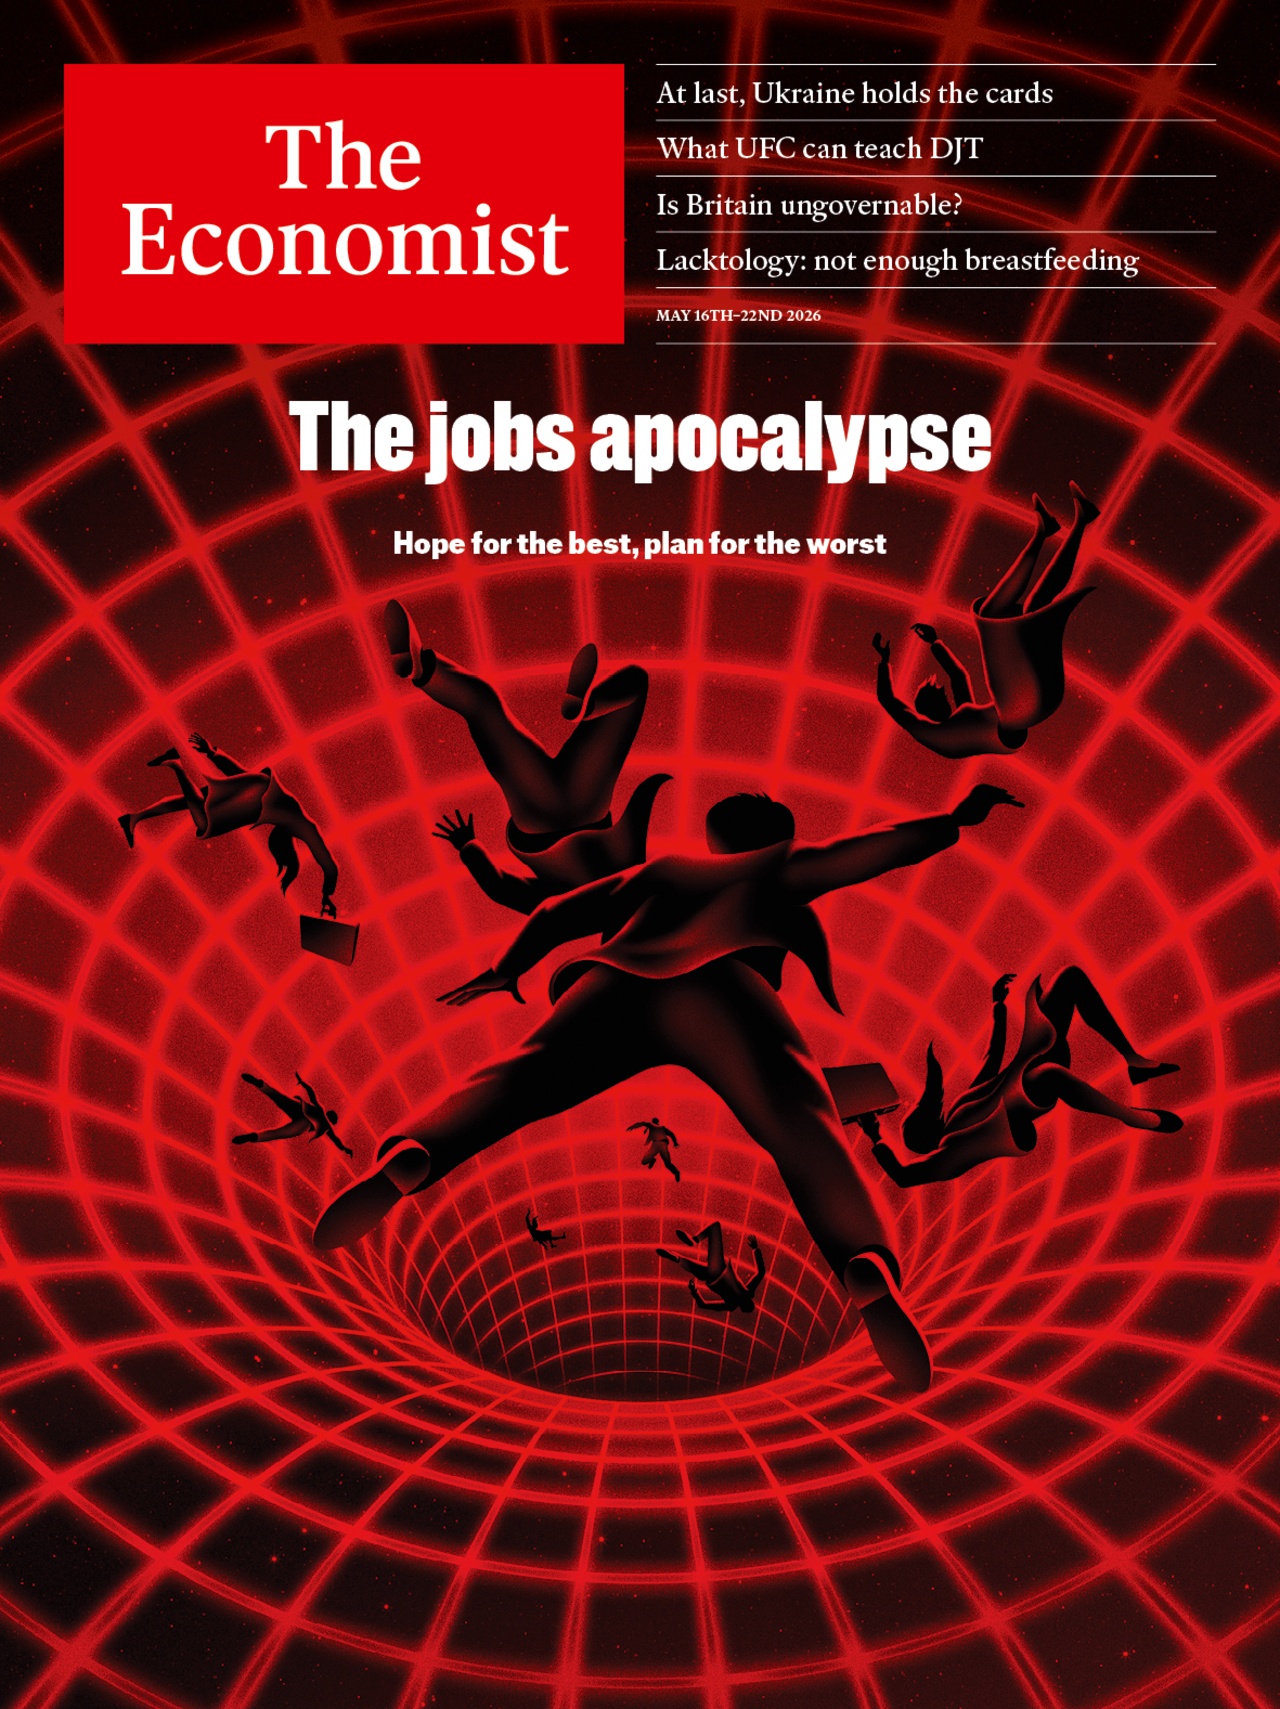
\includegraphics[height=5cm,keepaspectratio]{Economist_jobs_apocalypse.jpg}};
  \node<2->[rotate=3]  at (0, -0.3) {%
    \includegraphics[height=5cm,keepaspectratio]{{Atlantic_AI Has Ruined the Job Market}.JPG}};
  \node<3->[rotate=-2] at (4, 0.2) {%
    \includegraphics[height=5cm,keepaspectratio]{{Axios 2025 white collar bloodbath Amodei}.jpg}};
\end{tikzpicture}

\vspace{0.4em}
\end{frame}

% ---------------------------------------------------------------
\begin{frame}{Et spørsmål som kom inn på forhånd}
\begin{quote}
\large
«Juniorer og helt nyutdannede sliter med å komme inn på arbeidsmarkedet, i hvert fall innen IT-utvikling og kommunikasjon. Det skyldes neppe bare KI: usikkert marked, mindre konsulentinnleie i offentlig sektor, og seniorer som får gjort veldig mye alene med KI.

\medskip
Men vises virkelig ikke dette i statistikken?»
\end{quote}

\vspace{0.8em}
\footnotesize
Fra en deltaker i forkant av arrangementet, gjengitt med lett omskriving. Vi starter der: hva viser registerdataene for akkurat disse yrkene?
\end{frame}

% Yrkescase, én per slide, i stil med Yrkescase-delen på kiindeksen.no.
% Figurer: analysis/06_figures/plot_occ_cases_single.py
% (sesongjustert antall ansatte, indeksert til oktober 2022 = 100, privat sektor).

\begin{frame}{Programvareutviklere}
\centering
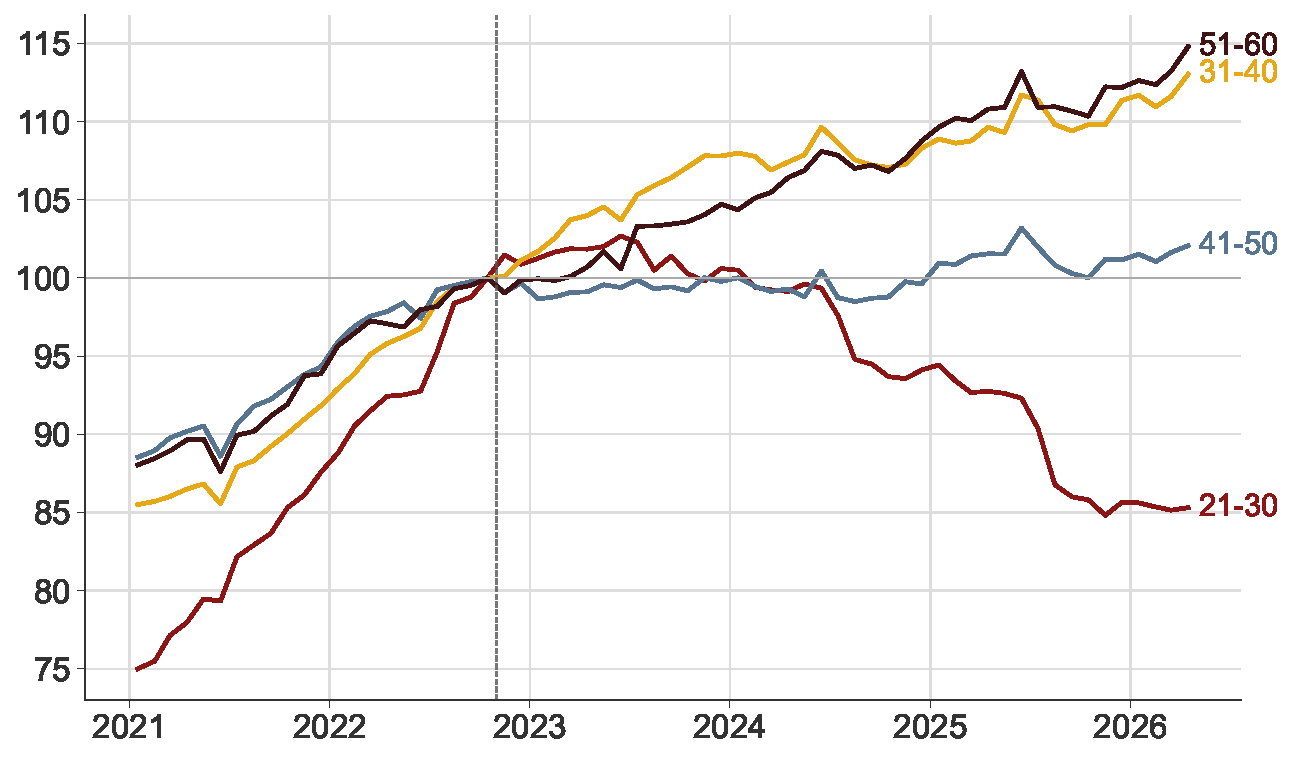
\includegraphics[height=5.4cm,keepaspectratio]{figure_case_utviklere_sa.pdf}

\vspace{0.15em}
\raggedright\scriptsize
Én linje per aldersgruppe; 100 = nivået i oktober 2022, måneden før ChatGPT. Sesongjustert, privat sektor. STYRK-08 2512 Programvareutviklere, 2513 Nett- og multimediautviklere, 2514 Applikasjonsprogrammerere, 2519 Andre programvare- og applikasjonsutviklere. Rundt 26\,000 ansatte (21--60 år) høsten 2022. Høy KI-eksponering (øverste femtedel).
\end{frame}

% ---------------------------------------------------------------
\begin{frame}{Informasjonsrådgivere}
\centering
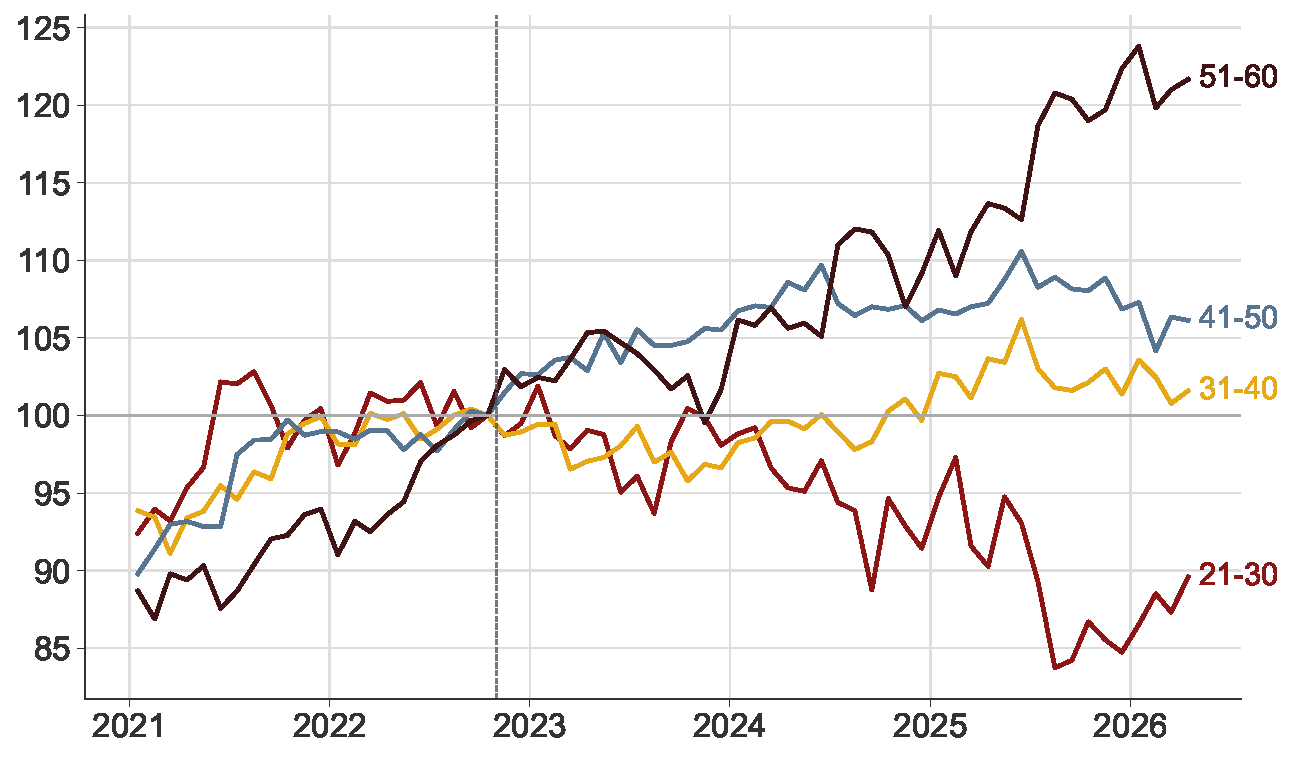
\includegraphics[height=5.8cm,keepaspectratio]{figure_case_informasjonsradgivere_sa.pdf}

\vspace{0.15em}
\raggedright\scriptsize
STYRK-08 2432 Informasjonsrådgivere: kommunikasjonsrådgivere, PR- og informasjonsmedarbeidere. Rundt 2\,700 ansatte i privat sektor høsten 2022; den offentlige delen av yrket inngår ikke. Høy KI-eksponering (øverste femtedel).
\end{frame}

% ---------------------------------------------------------------
\begin{frame}{Designyrker}
\centering
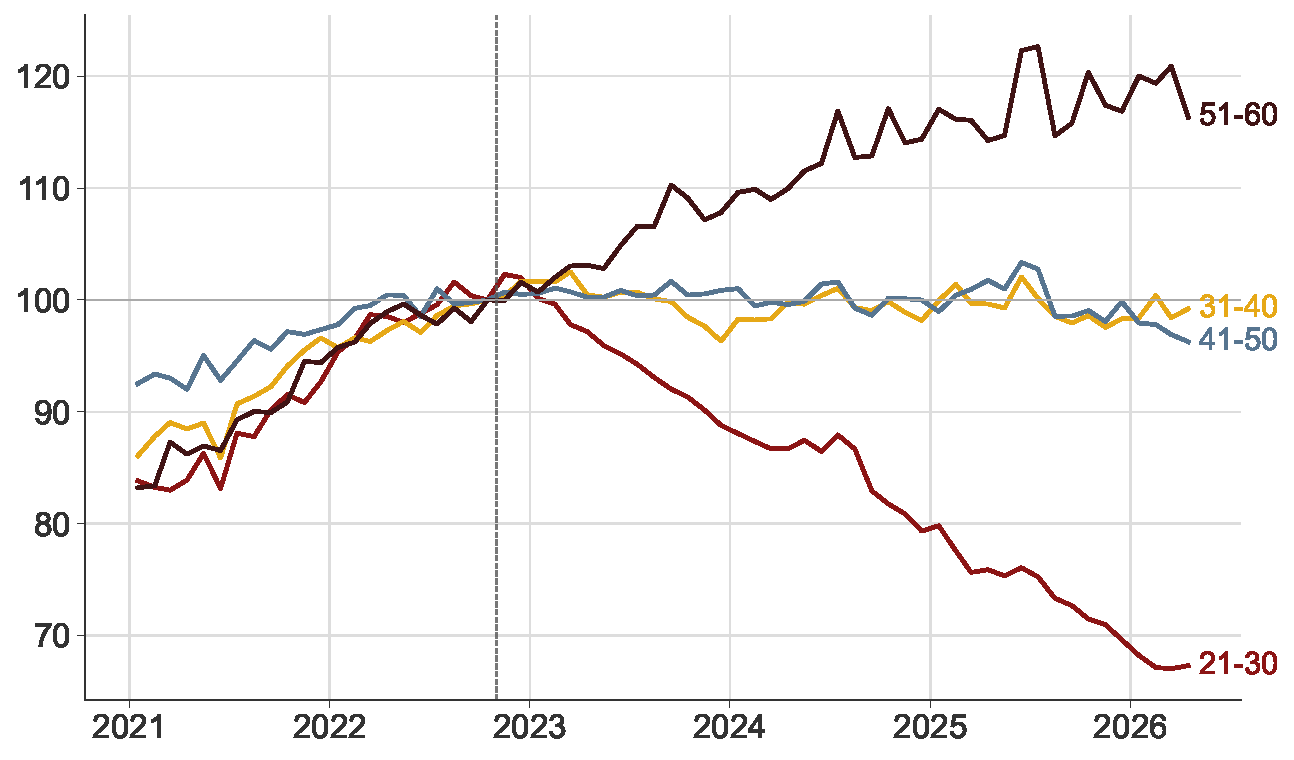
\includegraphics[height=6.1cm,keepaspectratio]{figure_case_designyrker_sa.pdf}

\vspace{0.15em}
\raggedright\scriptsize
STYRK-08 2163 Produkt- og klesdesignere og 2166 Grafiske- og multimediadesignere, sett under ett. Rundt 5\,600 ansatte høsten 2022. KI-eksponering i nest øverste femtedel.
\end{frame}

% ---------------------------------------------------------------
\begin{frame}{Kundebehandlere}
\centering
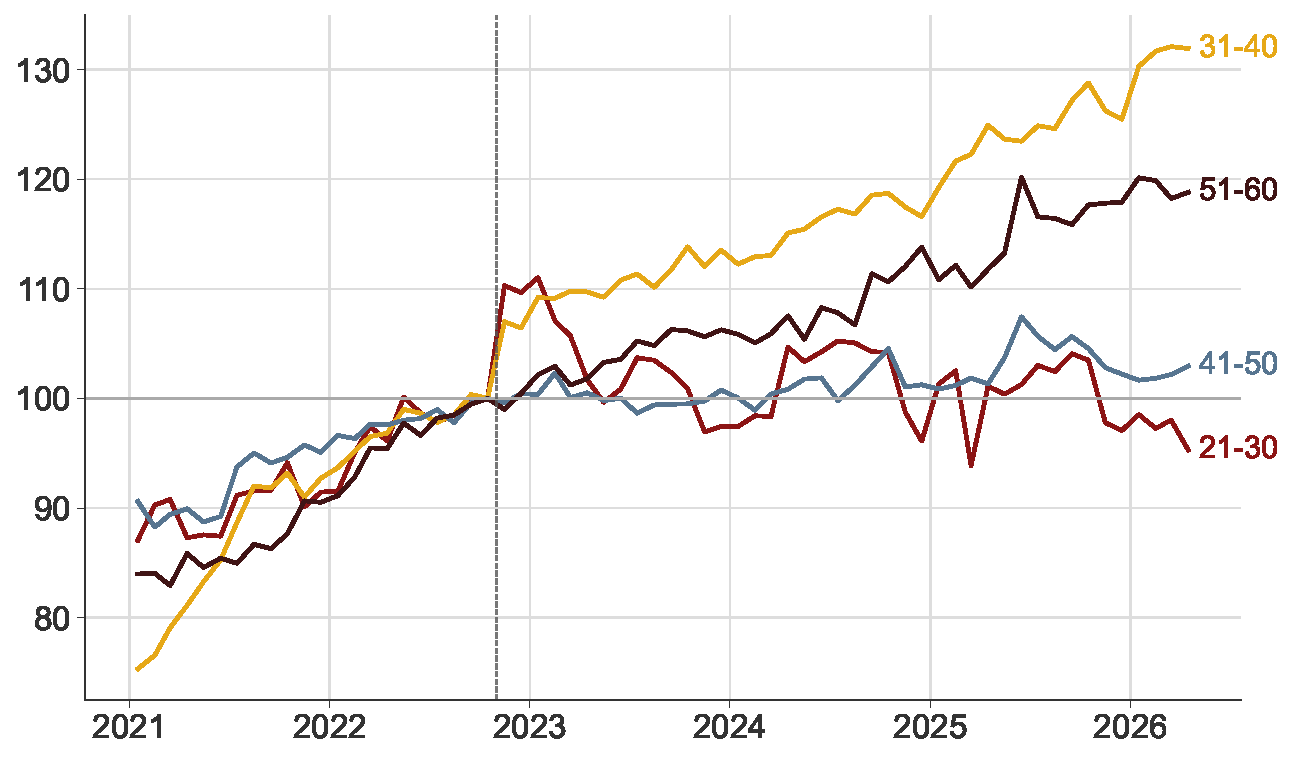
\includegraphics[height=6.1cm,keepaspectratio]{figure_case_kundebehandlere_sa.pdf}

\vspace{0.15em}
\raggedright\scriptsize
STYRK-08 4222 Kundesentermedarbeidere. Rundt 4\,000 ansatte høsten 2022; seriene for de eldste gruppene bygger på få personer og svinger mye. Høy KI-eksponering (øverste femtedel).
\end{frame}

% ---------------------------------------------------------------
\begin{frame}{Elektrikere}
\centering
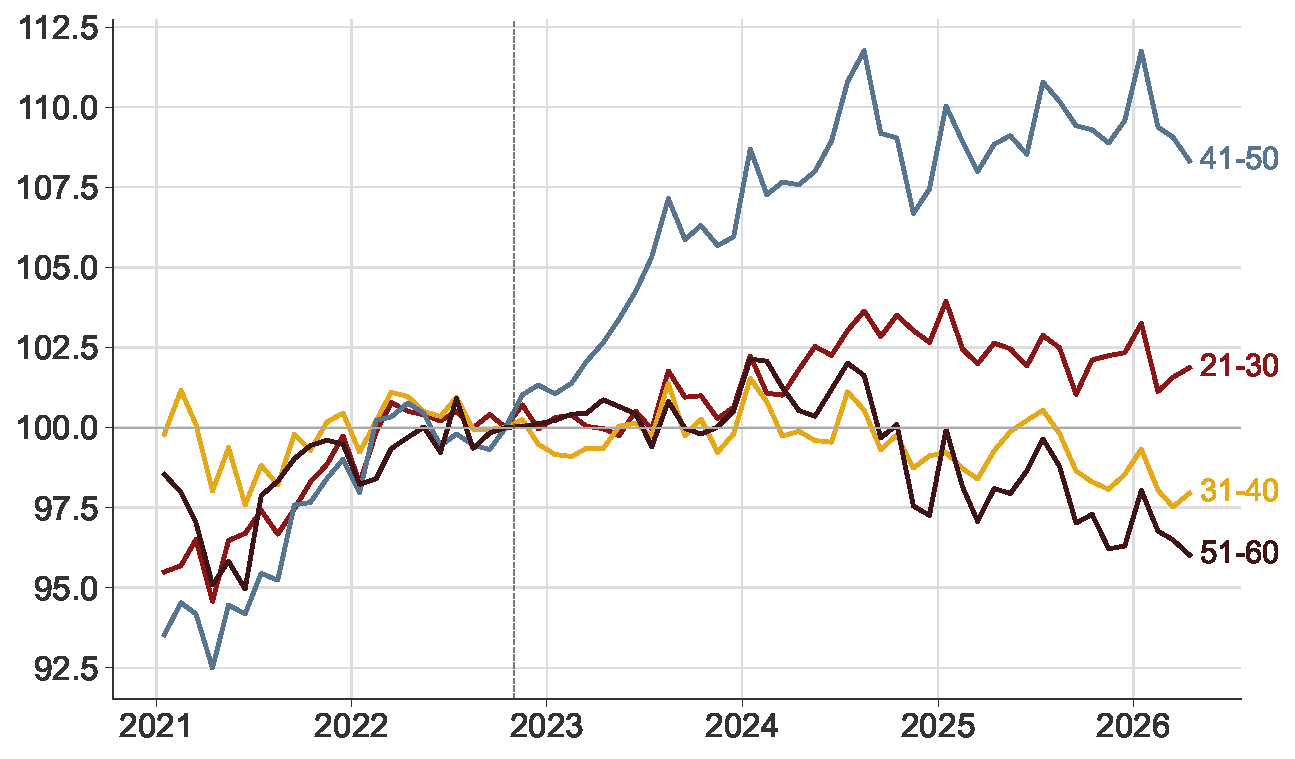
\includegraphics[height=6.1cm,keepaspectratio]{figure_case_elektrikere_sa.pdf}

\vspace{0.15em}
\raggedright\scriptsize
STYRK-08 7411 Elektrikere. Rundt 26\,000 ansatte høsten 2022. Håndverksyrke med lav KI-eksponering (nederste femtedel). Referanseyrke: her venter vi ikke utslag av KI.
\end{frame}

% ---------------------------------------------------------------
\begin{frame}{Hjemmehjelpere}
\centering
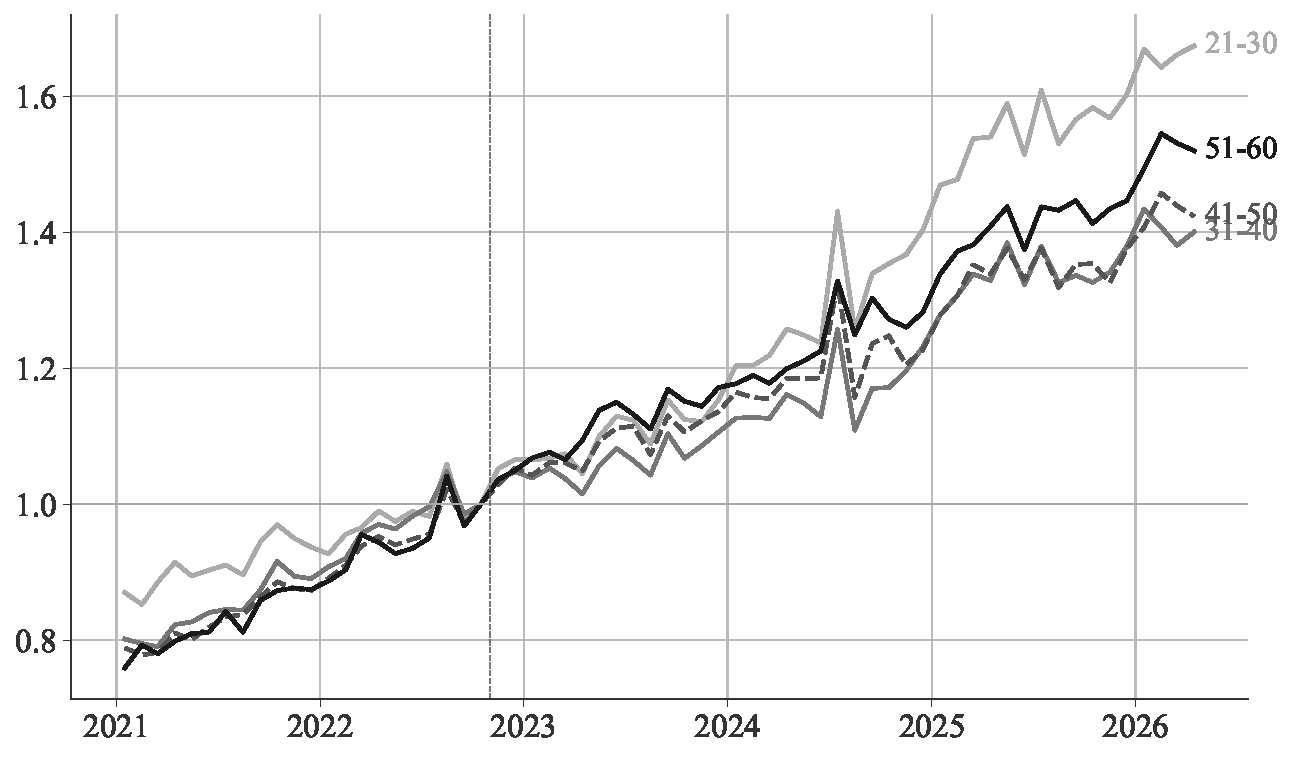
\includegraphics[height=6.1cm,keepaspectratio]{figure_case_hjemmehjelpere_sa.pdf}

\vspace{0.15em}
\raggedright\scriptsize
STYRK-08 5322 Hjemmehjelper. Rundt 9\,000 ansatte i privat sektor høsten 2022; den store kommunale delen av yrket inngår ikke. Lav KI-eksponering. Sterk vekst i alle aldersgrupper.
\end{frame}

% Hvordan vi måler: oppgaveperspektivet, indeksen, eksponeringsskår, gruppering.
% Illustrasjonsslidene er de samme som i presentation_no (TikZ-gjenskapinger
% av den private pptx-decken).

\begin{frame}{En jobb består av oppgaver som påvirkes ulikt}
\textcolor{illInk}{\textbf{Teknologi kan endre deler av jobben uten å erstatte hele.}}

\vspace{0.3em}
\centering
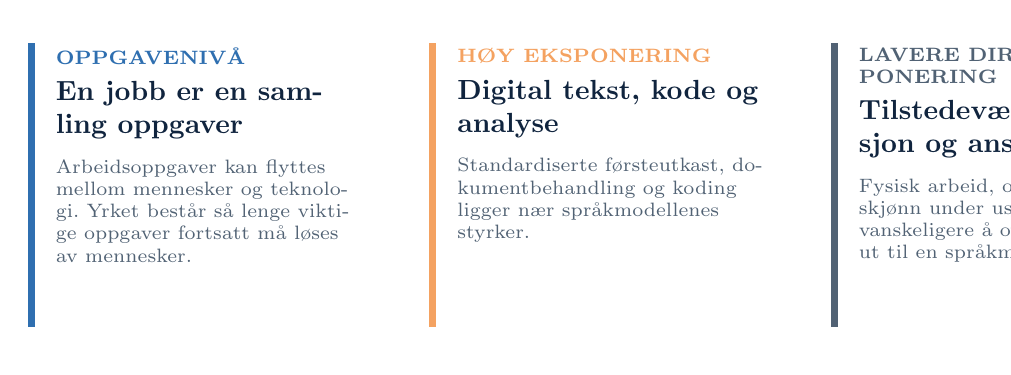
\begin{tikzpicture}
  \useasboundingbox (0,0.2) rectangle (\textwidth,-3.85);
  \illcard{(0.0,0)}{illBlue}{OPPGAVENIVÅ}{En jobb er en samling oppgaver}{Arbeidsoppgaver kan flyttes mellom mennesker og teknologi. Yrket består så lenge viktige oppgaver fortsatt må løses av mennesker.}
  \illcard{(5.1,0)}{illOrange}{HØY EKSPONERING}{Digital tekst, kode og analyse}{Standardiserte førsteutkast, dokumentbehandling og koding ligger nær språkmodellenes styrker.}
  \illcard{(10.2,0)}{illGray}{LAVERE DIREKTE EKSPONERING}{Tilstedeværelse, relasjon og ansvar}{Fysisk arbeid, omsorg og skjønn under usikkerhet er vanskeligere å overføre fullt ut til en språkmodell. Per nå.}
\end{tikzpicture}

\vspace{0.15em}
\illbanner{Rutinepregede inngangsoppgaver kan endres før hele yrker gjør det.}

\vspace{0.1em}
\raggedright\tiny\textcolor{illGray}{Kilder: Autor, Levy \& Murnane (2003); Acemoglu \& Autor (2011); Eloundou mfl.\ (2024); Brynjolfsson, Chandar \& Chen (2025).}
\end{frame}

% ---------------------------------------------------------------
\begin{frame}{Tre krefter trekker sysselsettingen i ulike retninger}
\vspace{0.3em}
\centering
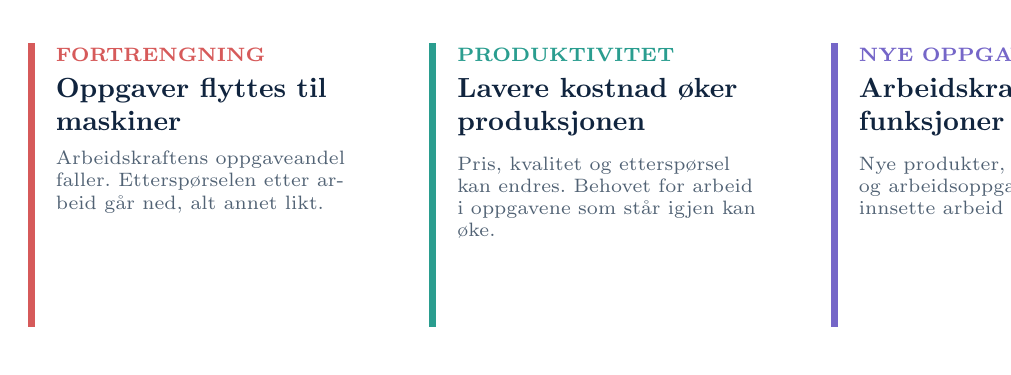
\begin{tikzpicture}
  \useasboundingbox (0,0.2) rectangle (\textwidth,-3.85);
  \illcard{(0.0,0)}{illRed}{FORTRENGNING}{Oppgaver flyttes til maskiner}{Arbeidskraftens oppgaveandel faller. Etterspørselen etter arbeid går ned, alt annet likt.}
  \illcard{(5.1,0)}{illTeal}{PRODUKTIVITET}{Lavere kostnad øker produksjonen}{Pris, kvalitet og etterspørsel kan endres. Behovet for arbeid i oppgavene som står igjen kan øke.}
  \illcard{(10.2,0)}{illPurple}{NYE OPPGAVER}{Arbeidskraft får nye funksjoner}{Nye produkter, kontrollbehov og arbeidsoppgaver kan gjeninnsette arbeid i produksjonen.}
\end{tikzpicture}

\vspace{0.15em}
\illbanner{Nettoeffekten følger ikke av hva modellen teknisk sett kan gjøre.}

\vspace{0.1em}
\raggedright\tiny\textcolor{illGray}{Rammeverk: Acemoglu og Restrepo (2019), Automation and New Tasks.}
\end{frame}

% ---------------------------------------------------------------
\begin{frame}{Fire ulike størrelser som ofte blandes sammen}
\vspace{0.4em}
\centering
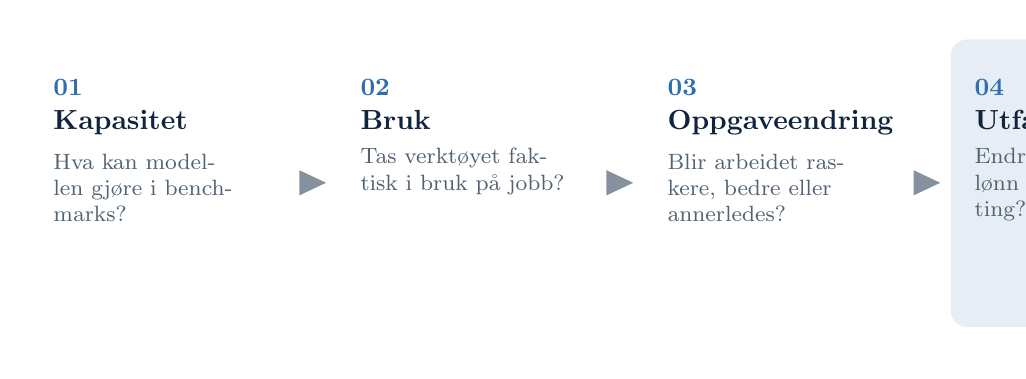
\begin{tikzpicture}
  \useasboundingbox (-0.2,0.5) rectangle (\textwidth,-3.6);
  \illstep{(0.0,0)}{01}{Kapasitet}{Hva kan modellen gjøre i benchmarks?}
  \illarrow{(3.25,-1.4)}
  \illstep{(3.9,0)}{02}{Bruk}{Tas verktøyet faktisk i bruk på jobb?}
  \illarrow{(7.15,-1.4)}
  \illstep{(7.8,0)}{03}{Oppgaveendring}{Blir arbeidet raskere, bedre eller annerledes?}
  \illarrow{(11.05,-1.4)}
  \illstepx{(11.7,0)}{04}{Utfall}{Endres ansettelser, lønn eller sysselsetting?}
\end{tikzpicture}

\vspace{0.8em}
\centering
\textcolor{illInk}{\textbf{KI-indeksen observerer det siste leddet: arbeidsmarkedsutfall i norske registerdata.}}

\vspace{0.4em}
\raggedright\tiny\textcolor{illGray}{Kilder: Narayanan \& Kapoor (2025); Eloundou mfl.\ (2024); Google (2026); kiindeksen.no.}
\end{frame}

% ---------------------------------------------------------------
\begin{frame}{Hva KI-indeksen måler}
\vspace{0.4em}
\centering
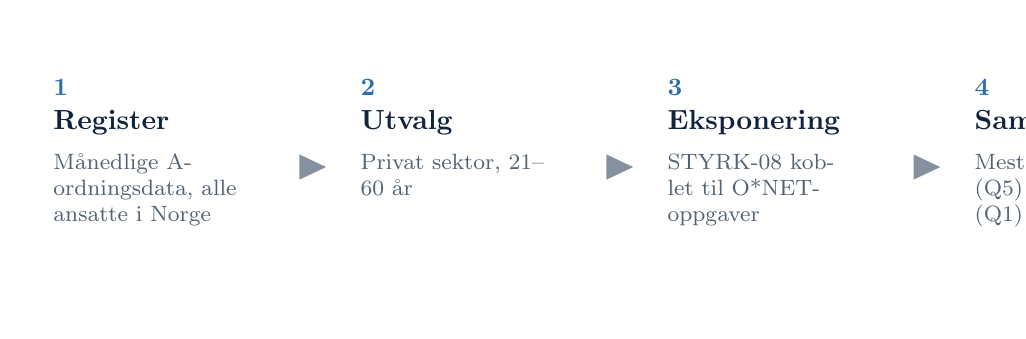
\begin{tikzpicture}
  \useasboundingbox (-0.2,0.5) rectangle (\textwidth,-3.1);
  \illstep{(0.0,0)}{1}{Register}{Månedlige A-ordningsdata, alle ansatte i Norge}
  \illarrow{(3.25,-1.2)}
  \illstep{(3.9,0)}{2}{Utvalg}{Privat sektor, 21--60 år}
  \illarrow{(7.15,-1.2)}
  \illstep{(7.8,0)}{3}{Eksponering}{STYRK-08 koblet til O*NET-oppgaver}
  \illarrow{(11.05,-1.2)}
  \illstep{(11.7,0)}{4}{Sammenligning}{Mest eksponert (Q5) mot minst (Q1)}
\end{tikzpicture}

\vspace{0.5em}
\illbanner{KI-indeksen: relativ sysselsettingsvekst i mest (Q5) mot minst (Q1) eksponert, snitt av siste tre måneder mot oktober 2022.}

\vspace{0.2em}
\raggedright\tiny\textcolor{illGray}{Kilder: kiindeksen.no; Hernæs \& Kostøl (2026).}
\end{frame}

% ---------------------------------------------------------------
\begin{frame}{Eksponering måles på konkrete O*NET-oppgaver}
\begin{columns}[T,onlytextwidth]
\begin{column}{0.36\textwidth}
  {\bfseries\textcolor{illBlue}{O*NET}}

  \vspace{0.5em}
  {\footnotesize\textcolor{illGray}{Datasett fra US Department of Labor som beskriver rundt 1\,000 yrker med konkrete oppgaver. Eloundou mfl.\ vurderte hver oppgave for alle yrker.}}

  \vspace{1.4em}
  {\small\bfseries\textcolor{illInk}{KI-indeksens yrkesskår = Core-vektet gjennomsnitt av oppgavepoengene}}

  \vspace{0.4em}
  {\footnotesize\textcolor{illGray}{Core-oppgaver teller 2; Supplemental-oppgaver teller 1.}}
\end{column}
\begin{column}{0.60\textwidth}
  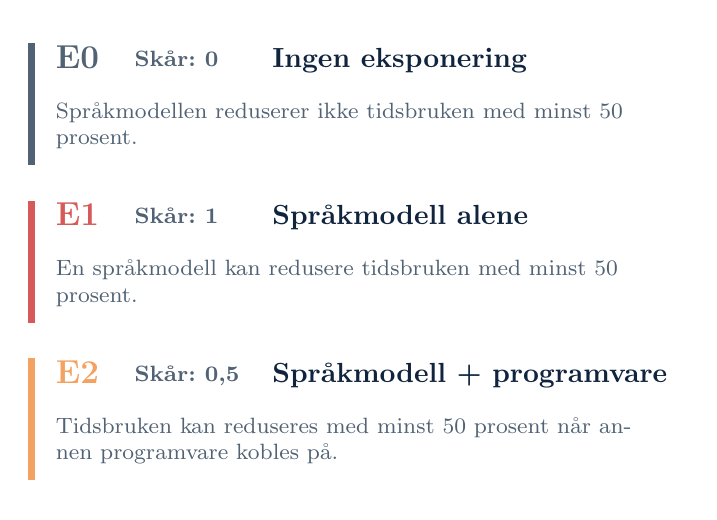
\begin{tikzpicture}
    \useasboundingbox (0,0.2) rectangle (8.4,-5.7);
    \illerow{(0,0)}{illGray}{E0}{Skår: 0}{Ingen eksponering}{Språkmodellen reduserer ikke tidsbruken med minst 50 prosent.}
    \illerow{(0,-2.0)}{illRed}{E1}{Skår: 1}{Språkmodell alene}{En språkmodell kan redusere tidsbruken med minst 50 prosent.}
    \illerow{(0,-4.0)}{illOrange}{E2}{Skår: 0,5}{Språkmodell + programvare}{Tidsbruken kan reduseres med minst 50 prosent når annen programvare kobles på.}
  \end{tikzpicture}
\end{column}
\end{columns}

\vspace{0.2em}
\raggedright\tiny\textcolor{illGray}{Kilder: O*NET Resource Center; Eloundou mfl.\ (Science, 2024).}
\end{frame}

% ---------------------------------------------------------------
\begin{frame}{Fra oppgaver til skår: informasjonsrådgivere}
\raggedright\scriptsize STYRK 2432 $\cdot$ O*NET 27-3031.00 $\cdot$ én-til-én-kobling gjennom SOC 2018 og SOC 2010

\vspace{0.3em}
\centering\tiny
\setlength{\tabcolsep}{3pt}
\renewcommand{\arraystretch}{1.12}
\begin{tabular}{p{4.9cm}cc @{\hspace{0.5cm}} p{5.3cm}cc}
\toprule
O*NET-oppgave & $E$ & $\beta$ & O*NET-oppgave & $E$ & $\beta$ \\
\midrule
\rO{Svare medier eller finne talsperson}{$E_2$}{0,5}        & \rO{Arrangere opptredener og arrangementer}{$E_2$}{0,5} \\
\rO{Planlegge kommunikasjonsprogrammer}{$E_2$}{0,5}         & \rO{Gjennomføre markeds- og opinionsundersøkelser}{$E_2$}{0,5} \\
\rR{Oppdatere nettside og sosiale medier}{$E_1$}{1}         & \rO{Formidle miljø- og samfunnstiltak}{$E_2$}{0,5} \\
\rR{Skrive pressemeldinger og medietekst}{$E_1$}{1}         & \rO{Koordinere reklame- og kampanjeproduksjon}{$E_2$}{0,5} \\
Bygge relasjoner til interessegrupper & $E_0$ & 0            & \rO{Planlegge kampanjer med byråer og medier}{$E_2$}{0,5} \\
\rO{Rådgi ledere om trender og interesser}{$E_2$}{0,5}      & \rR{Skrive eller holde taler}{$E_1$}{1} \\
\rO{Trene talspersoner i kommunikasjon}{$E_2$}{0,5}         & \rO{Håndtere offentlig respons ved hendelser (supp.)}{$E_2$}{0,5} \\
\rO{Utvikle PR-strategier}{$E_2$}{0,5}                      & \rO{Markedsføre miljøteknologi og -tjenester (supp.)}{$E_2$}{0,5} \\
\rR{Redigere interne og eksterne publikasjoner}{$E_1$}{1}   & \rO{Kjøpe annonseplass og sendetid (supp.)}{$E_2$}{0,5} \\
\midrule
\multicolumn{6}{l}{\textbf{18 oppgaver: 1 $E_0$ \; 4 $E_1$ \; 13 $E_2$ \quad Core $\times$ 2, Supplemental $\times$ 1 \quad yrkes-$\beta$ = 0,591 \quad øverste femtedel (Q5)}} \\
\bottomrule
\end{tabular}

\vspace{0.3em}
\raggedright\tiny\textcolor{illGray}{Kilde: O*NET, Eloundou mfl.\ (2024) og prosjektets SOC--ISCO/STYRK-krysskobling. Oppgavetekstene er oversatt fra O*NET.}
\end{frame}

% ---------------------------------------------------------------
\begin{frame}{397 yrker rangeres og deles i fem like store grupper}
\begin{columns}[T,onlytextwidth]
\begin{column}{0.47\textwidth}
{\small\bfseries\textcolor{illGray}{Q1: minst eksponert}}

\vspace{0.4em}
\small
Renholdere \\ Elektrikere \\ Bilmekanikere \\ Rørleggere
\end{column}
\begin{column}{0.47\textwidth}
{\small\bfseries\textcolor{illBlue}{Q5: mest eksponert}}

\vspace{0.4em}
\small
Selgere (engros) \\ Kontormedarbeidere \\ Systemanalytikere \\ Programvareutviklere \\ Regnskapsførere
\end{column}
\end{columns}

\vspace{1.0em}
\begin{itemize}\setlength{\itemsep}{4pt}
  \item Hvert yrke får sin skår, som informasjonsrådgiverne fikk 0,591.
  \item Yrkene rangeres og deles i fem like store grupper, fra minst til mest eksponert.
  \item KI-indeksen sammenligner sysselsettingsveksten i den øverste og den nederste gruppen.
\end{itemize}
\end{frame}

% Det samlede bildet: ingen jobbkrise, dashbordet, unge samlet.

\begin{frame}{Samlet: de mest eksponerte yrkene har klart seg som de minst eksponerte}
\centering
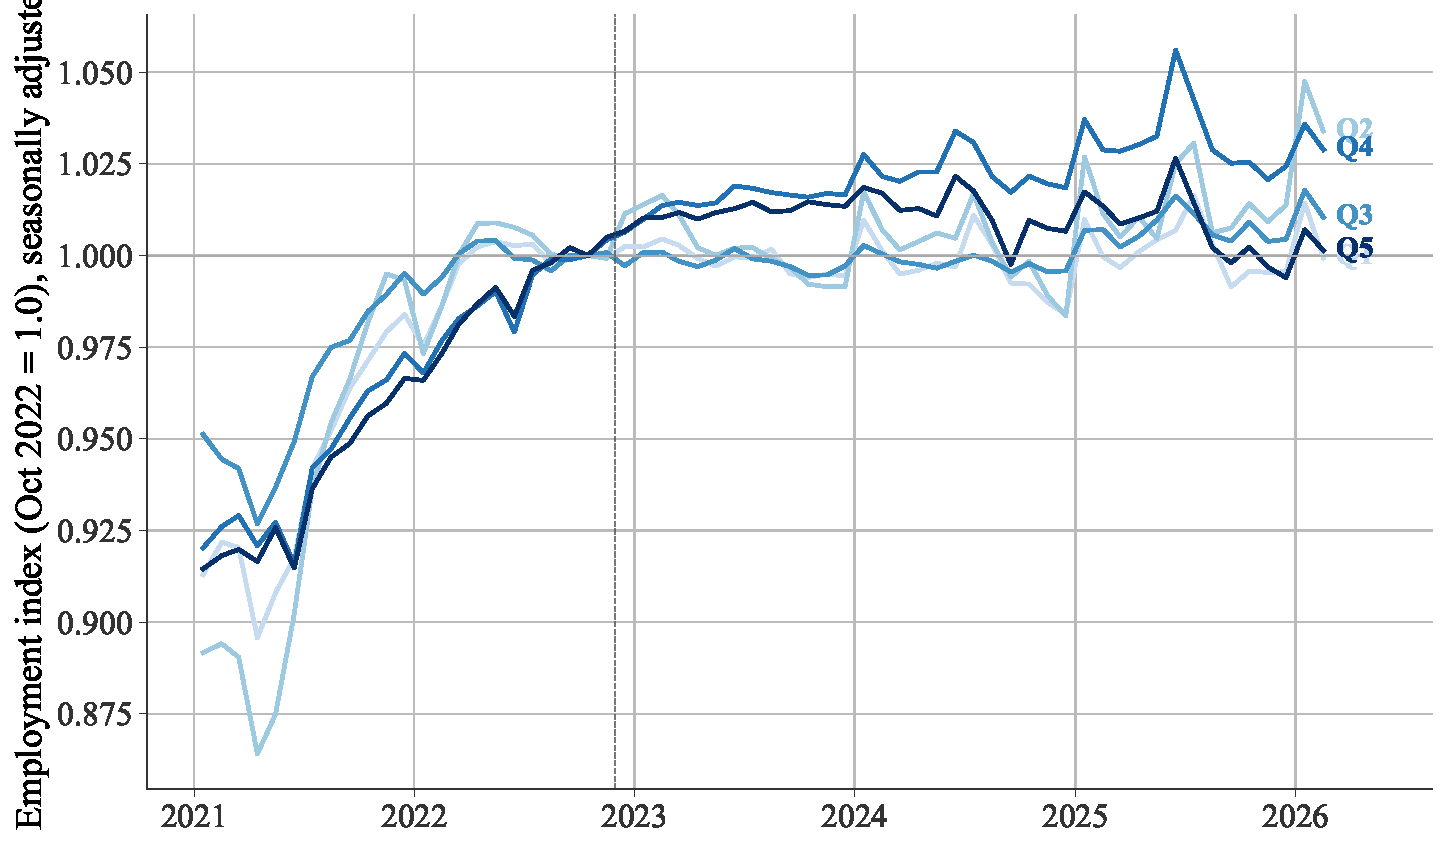
\includegraphics[height=5.8cm,keepaspectratio]{figure_emp_byexposure_sa.pdf}

\vspace{0.2em}
\footnotesize
Sysselsetting i femdelene fra forrige slide, 21--60 år, privat sektor, sesongjustert, oktober 2022 = 1. KI-indeksen står i dag på $+0{,}5$ prosentpoeng, godt innenfor usikkerhetsbåndet.
\end{frame}

% ---------------------------------------------------------------
\begin{frame}{kiindeksen.no}
\centering
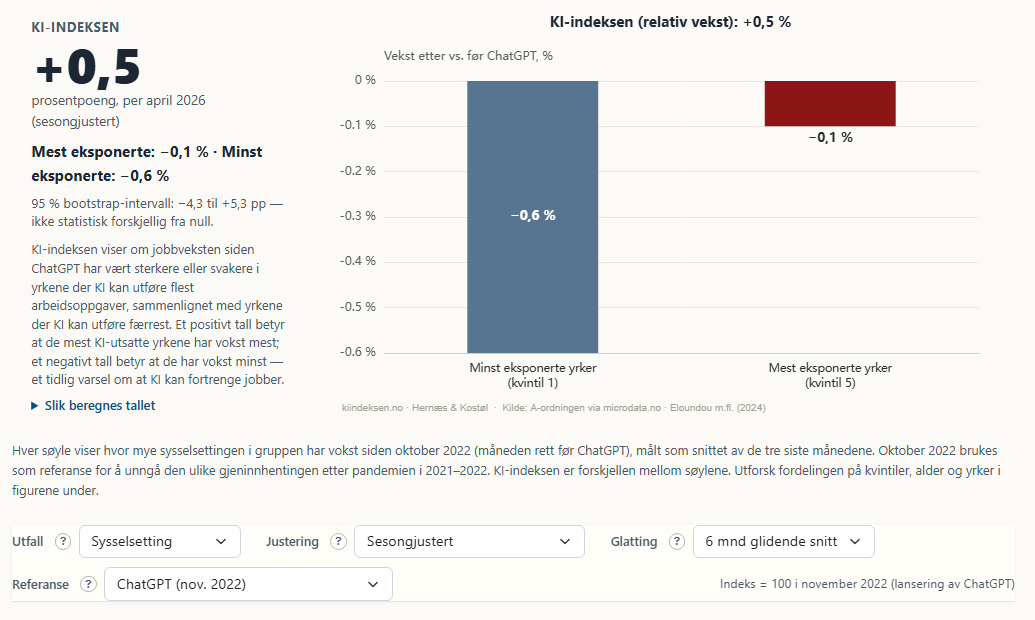
\includegraphics[height=5.9cm,keepaspectratio]{kiindeksen_screenshot.png}

\vspace{0.2em}
\footnotesize
Offentlig dashbord, oppdateres månedlig. Der kan du selv velge utfall, aldersgruppe, enkeltyrker, sesongjustering og glatting.
\end{frame}

% ---------------------------------------------------------------
\begin{frame}{Heller ikke de yngste faller bak som gruppe}
\centering
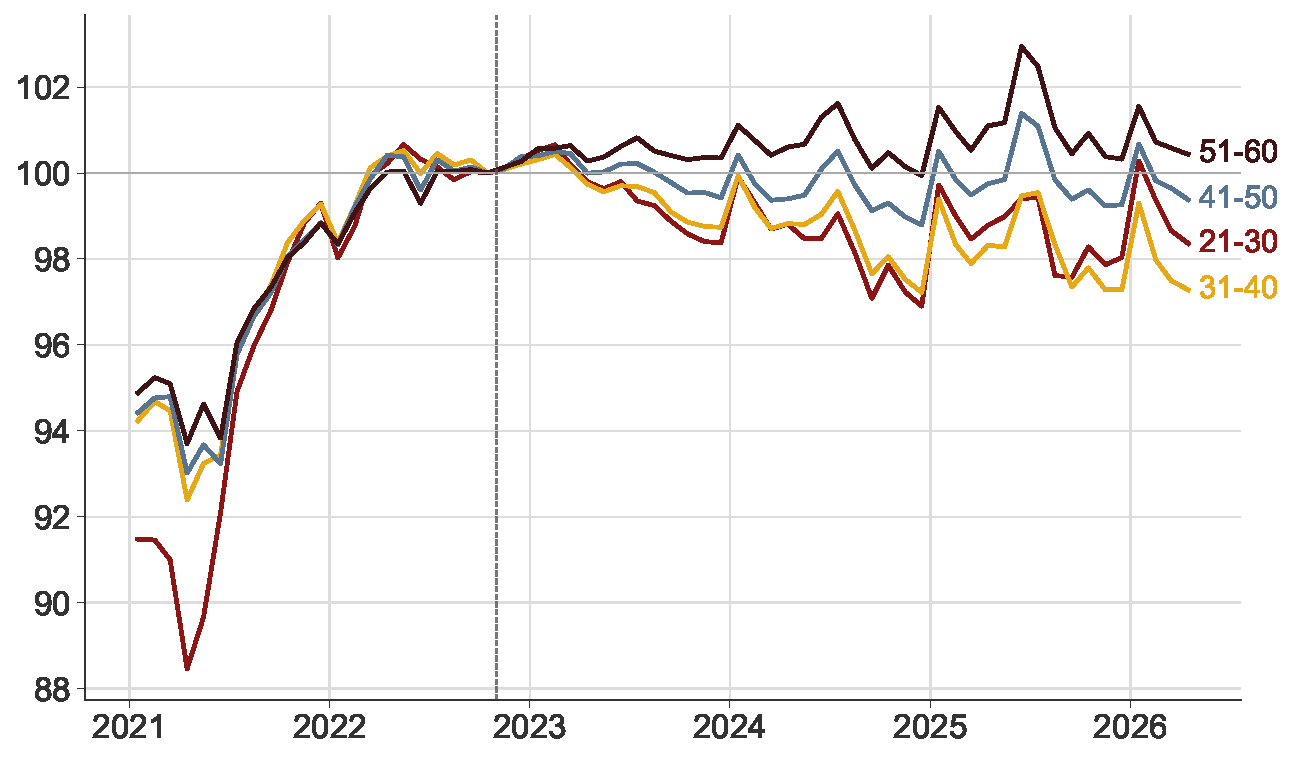
\includegraphics[height=5.8cm,keepaspectratio]{figure_case_alder_sa.pdf}

\vspace{0.2em}
\footnotesize
Sysselsetting per aldersgruppe, alle yrker, privat sektor, sesongjustert, 100 = oktober 2022. De yngste ligger et par indekspoeng under toppen fra 2022, men følger de andre gruppene tett.
\end{frame}

% Svar på forhåndsspørsmålet, avgrensninger, policy, råd til unge, avslutning.

\begin{frame}{Vises det i statistikken? Ja, noe. Men ikke bredt.}
\begin{columns}[T,onlytextwidth]
\begin{column}{0.48\textwidth}
{\bfseries\textcolor{illInk}{Dette ser vi}}

\vspace{0.4em}
\small
\begin{itemize}\setlength{\itemsep}{5pt}
  \item De yngste faller i flere høyeksponerte yrker siden oktober 2022: utviklere $-15\,\%$, designyrker $-32\,\%$, informasjonsrådgivere $-10\,\%$ (per innbygger). De eldste i de samme yrkene vokser.
  \item Anthropic ser det samme i egne data: rundt 14\,\% lavere jobbstartrate for unge inn i eksponerte yrker (2026).
\end{itemize}
\end{column}
\begin{column}{0.48\textwidth}
{\bfseries\textcolor{illInk}{Dette ser vi ikke}}

\vspace{0.4em}
\small
\begin{itemize}\setlength{\itemsep}{5pt}
  \item Noe bredt fall i de mest eksponerte yrkene samlet, eller for 21--30-gruppen samlet.
  \item Hva som driver unge-fallet: erstattet av KI, junioroppgaver som forsvinner, strengere erfaringskrav eller seniorer som rekker mer. Der er «den perfekte stormen» av renter, konsulentkutt og normalisering etter pandemien også med.
\end{itemize}
\end{column}
\end{columns}

\vspace{0.6em}
\centering
\textcolor{illInk}{\textbf{Derfor følger vi det månedlig.}}
\end{frame}

% ---------------------------------------------------------------
\begin{frame}{Hva vi ikke sier}
\small
\begin{itemize}\setlength{\itemsep}{6pt}
  \item Indeksen er et beskrivende vekstgap, ikke en målt årsakseffekt av KI.
  \item Den dekker privat sektor; offentlig sektor inngår ikke i hovedtallet.
  \item Vi observerer utfall per yrke. Oppgaveinnholdet kan endre seg mye uten at yrkeskoden gjør det, og nye KI-roller kan være skjult i gamle koder.
  \item Yrkesstandardene er gamle: STYRK-08 er fra 2011 og bygger på ISCO-08 fra 2008, med en grunnmodell som går tilbake til ISCO-88. O*NET-oppgavene er amerikanske, vurdert i 2023. Arbeidsinnholdet i norske yrker kan avvike.
  \item Det bøter vi på slik: grove femdeler heller enn fininndeling, kryssjekk mot uavhengige mål som rangerer de samme yrkene høyt, og måling av faktiske utfall. Feil i kodingen visker ut forskjeller heller enn å skape dem.
\end{itemize}
\end{frame}

% ---------------------------------------------------------------
\begin{frame}{Politikk som treffer omstillingen}
\footnotesize
\setlength{\tabcolsep}{6pt}
\renewcommand{\arraystretch}{1.5}
\begin{tabular}{p{3.6cm} p{7.4cm} p{2.6cm}}
\textbf{\textcolor{illInk}{Sikre omskolering og inngang til jobb}} & Dagpenger under utdanning til mangelyrker, inntektssikret utdanningspermisjon, flere lønnstilskuddsplasser og stabilt statlig inntak av nyutdannede. & {\tiny\textcolor{illGray}{Kostøl \& Harang, DN 29.7.2026}} \\
\textbf{\textcolor{illInk}{Endre skatteinsentivene}} & Gjør ansettelser, opplæring og arbeidskomplementær KI mer konkurransedyktig mot ren automatisering og kjøp av maskinkapasitet. & {\tiny\textcolor{illGray}{Harang \& Kostøl, DN 29.6.2026; Acemoglu \& Johnson 2023; Brynjolfsson 2022}} \\
\textbf{\textcolor{illInk}{Finansier nye opplæringsstiger}} & Støtt sertifisert bedriftsopplæring, bransjefelles treningsløp og praksisordninger når juniorarbeidet ikke lenger finansierer læringen. & {\tiny\textcolor{illGray}{Garicano 2025}} \\
\textbf{\textcolor{illInk}{Forbered institusjonene på flere utfall}} & Følg teknologisk kapasitet, bruk og arbeidsmarkedsutfall; stresstest skatt og sikkerhetsnett og gjør tiltakene skalerbare. & {\tiny\textcolor{illGray}{Korinek 2023}} \\
\end{tabular}
\end{frame}

% ---------------------------------------------------------------
\begin{frame}{Råd til unge: skaff faglig dybde og erfaring tidlig}
\footnotesize
\setlength{\tabcolsep}{6pt}
\renewcommand{\arraystretch}{1.5}
\begin{tabular}{p{3.9cm} p{7.1cm} p{2.6cm}}
\textbf{\textcolor{illInk}{Bruk KI på virkelige oppgaver}} & Dokumenter arbeidsmåten, finn feil og kontroller kildene. & {\tiny\textcolor{illGray}{Mollick 2023; Brynjolfsson 2026}} \\
\textbf{\textcolor{illInk}{Behold selvstendig faglig arbeid}} & Gjør et eget forsøk først. Lær premisser, metode og dømmekraft. & {\tiny\textcolor{illGray}{Goldsmith-Pinkham 2026; Gans 2026}} \\
\textbf{\textcolor{illInk}{Fullfør grad eller fagbrev}} & Velg en grunnmur som åpner flere jobber, og lær KI i selve faget. & {\tiny\textcolor{illGray}{Deming 2025; Sigelman 2026}} \\
\textbf{\textcolor{illInk}{Prioriter praksis og mentorering}} & Spør hvordan arbeidsplassen trener juniorer når rutineoppgavene blir færre. & {\tiny\textcolor{illGray}{Brynjolfsson 2026; Garicano 2025}} \\
\textbf{\textcolor{illInk}{Vis hva du kan gjøre}} & Bygg noen gjennomførte arbeider og kombiner teknikk med samarbeid og kommunikasjon. & {\tiny\textcolor{illGray}{Bryan 2026; Erdil \& Besiroglu 2025}} \\
\end{tabular}
\end{frame}

% ---------------------------------------------------------------
\begin{frame}{Følg med videre}
\centering
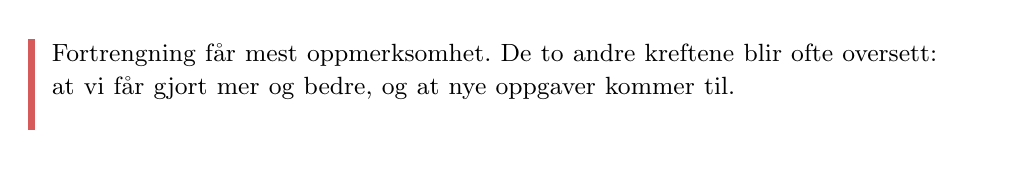
\begin{tikzpicture}
  \useasboundingbox (0,0.2) rectangle (\textwidth,-1.3);
  \node[anchor=north west, text width=0.94\textwidth, inner sep=0pt] at (0.3,0) {%
    \small Fortrengning får mest oppmerksomhet. De to andre kreftene blir ofte oversett: at vi får gjort mer og bedre, og at nye oppgaver kommer til.};
  \fill[illRed] (0,0.05) rectangle (0.09,-1.1);
\end{tikzpicture}

\vspace{0.6em}
{\LARGE\bfseries\textcolor{illInk}{kiindeksen.no}}

\vspace{0.8em}
\large
Oppdateres hver måned når nye registerdata kommer.

\vspace{1.2em}
\footnotesize
Engelsk versjon: kiindeksen.no/en \quad $\cdot$ \quad Hernæs (Frischsenteret) og Kostøl (Handelshøyskolen BI)
\end{frame}

% ---------------------------------------------------------------
\begin{frame}{Referanser (1/2)}
\scriptsize
\begin{columns}[T,onlytextwidth]
\begin{column}{0.48\textwidth}
\begin{itemize}\setlength{\itemsep}{2pt}
  \item Acemoglu, D.\ og D.\ Autor (2011): Skills, Tasks and Technologies. \emph{Handbook of Labor Economics}.
  \item Acemoglu, D.\ og S.\ Johnson (2023): Rebalancing AI. \emph{IMF Finance \& Development}, desember 2023.
  \item Acemoglu, D.\ og P.\ Restrepo (2019): Automation and New Tasks. \emph{Journal of Economic Perspectives}.
  \item Anthropic (2026): Labor Market Impacts of AI: A New Measure and Early Evidence (Massenkoff og McCrory).
  \item Autor, D., F.\ Levy og R.\ Murnane (2003): The Skill Content of Recent Technological Change. \emph{Quarterly Journal of Economics}.
  \item Brynjolfsson, E.\ (2022): The Turing Trap. \emph{Daedalus}.
  \item Brynjolfsson, E., B.\ Chandar og R.\ Chen (2025): Canaries in the Coal Mine? Arbeidsnotat, Stanford Digital Economy Lab.
\end{itemize}
\end{column}
\begin{column}{0.48\textwidth}
\begin{itemize}\setlength{\itemsep}{2pt}
  \item Eloundou, T., S.\ Manning, P.\ Mishkin og D.\ Rock (2024): GPTs are GPTs. \emph{Science}.
  \item Google (2026): AI \& Economy ATLAS v1.0: Mapping Gemini Usage in the Economy.
  \item Hernæs, Ø.\ og A.\,R.\ Kostøl (2026): KI-indeksen. kiindeksen.no.
  \item Korinek, A.\ (2023): Scenario Planning for an AGI Future. \emph{IMF Finance \& Development}, desember 2023.
  \item Narayanan, A.\ og S.\ Kapoor (2025): AI as Normal Technology. Knight First Amendment Institute.
  \item SSB (2011): Standard for yrkesklassifisering (STYRK-08). Notater 17/2011.
  \item O*NET Resource Center, U.S.\ Department of Labor.
  \item A-ordningen via microdata.no (SSB/Sikt/NSD).
\end{itemize}
\end{column}
\end{columns}
\end{frame}

% ---------------------------------------------------------------
\begin{frame}{Referanser (2/2): kronikker, essays og intervjuer}
\scriptsize
\begin{columns}[T,onlytextwidth]
\begin{column}{0.48\textwidth}
\begin{itemize}\setlength{\itemsep}{2pt}
  \item Kostøl, A.\,R.\ og F.\,N.\ Harang (2026): KI og det stille utenforskapet. Kronikk, \emph{Dagens Næringsliv}, 29.\ juli 2026.
  \item Harang, F.\,N.\ og A.\,R.\ Kostøl (2026): Maskiner må løfte mennesker. Kronikk, \emph{Dagens Næringsliv}, 29.\ juni 2026.
  \item Garicano, L.\ (2025): AI's Becker Problem. Essay, juli 2025.
  \item Mollick, E.\ (2023): On-boarding Your AI Intern. Essay, \emph{One Useful Thing}, mai 2023.
  \item Goldsmith-Pinkham, P.\ (2026): Research in the Time of AI. Essay, mars 2026.
  \item Gans, J.\ (2026): Journopoclypse! Essay, mars 2026.
\end{itemize}
\end{column}
\begin{column}{0.48\textwidth}
\begin{itemize}\setlength{\itemsep}{2pt}
  \item Brynjolfsson, E.\ (2026): intervju, \emph{Silicon Valley Girl}, juli 2026.
  \item Deming, D.\ (2025): intervju, \emph{Managing the Future of Work} (Harvard Business School), februar 2025.
  \item Sigelman, M.\ (2026): intervju, \emph{The Ongoing Transformation}, april 2026.
  \item Bryan, K.\ (2026): intervju, \emph{Justified Posteriors}, juni 2026.
  \item Erdil, E.\ og T.\ Besiroglu (2025): intervju, \emph{Dwarkesh Podcast}, april 2025.
\end{itemize}

\vspace{0.5em}
Policy- og råd-slidene gjengir forslag fra disse kildene; de er ikke evaluert som én samlet pakke.
\end{column}
\end{columns}
\end{frame}


\end{document}
